\section{Experiment Implementation Details on \benchname}
\label{sec:appx_imp_detail}

\subsection{Training Details for SAM2Act+}
\label{sec:sam2act}

We implement the SAM2Act+ architecture following the two-stage training pipeline described in the original paper~\cite{fang2025sam2act}. 
Specifically, we first pretrain the SAM2 backbone without temporal connections, and then fine-tune the memory attention module. 
Each stage is trained for 40k steps on our dataset. 
Training is conducted on four NVIDIA A40 GPUs for approximately 2.5 days per stage. 
The detailed training configurations and hyperparameters are provided in Table~\ref{tab:sam2actplus_train_hparams}.

\paragraph{Discrete Actions.}
A core design choice in SAM2Act+ is to operate in a \textbf{discrete action space} rather than predicting dense continuous actions. 
Our dataset also provides waypoint-based actions at keyframes, which are compatible with this formulation. 
However, due to the limitations of discrete action parameterization, performance degrades on tasks requiring precise continuous control, such as \textit{StopCube} and \textit{InsertPeg}. 
For the remaining tasks, the discrete actions are sufficient. 
Once the model predicts a waypoint, the ManiSkill simulator will invoke an internal motion planner to execute the action.

\paragraph{Video-based Observation Input.}
The original SAM2Act+ architecture does not include a dedicated mechanism for ingesting demonstration videos as conditional input. 
To support video-conditioned tasks, we treat the demonstration video as part of the action prediction process during training. 
At test time, we first roll out the demonstration video through SAM2Act+ to prefill its memory bank without interacting with the simulator. 
After memory initialization, the agent begins execution using the current observation, following the same protocol adopted in MemoryBench.

Our code for adapting SAM2Act+ can be found at \url{https://anonymtest1.github.io/}

\begin{table}[h]
\centering
\small
\caption{Training hyperparameters for SAM2Act and SAM2Act+.}
\label{tab:sam2actplus_train_hparams}
\begin{tabular}{lcc}
\toprule
\textbf{Hyperparameters} & \textbf{SAM2Act Training} & \textbf{SAM2Act+ Training} \\
\midrule
batch size  & 48 & 80 \\
learning rate & $6.0\times10^{-4}$ & $1.0\times10^{-4}$ \\
optimizer & LAMB  & LAMB \\
learning rate schedule & warmup + cosine & warmup + cosine \\
weight decay & $1\times10^{-4}$ & $1\times10^{-4}$ \\
warmup steps & 2000 & 2000 \\
total steps & 40K & 40K \\
training epochs & 10 & 10 \\
LoRA rank & 16 & 16 \\
data distribution & task uniform & demo uniform temporal\\
\bottomrule
\end{tabular}
\end{table}





\clearpage
\subsection{VLM Subgoal Prediction and Prompts}
\label{sec:VLM_subgoal}

Language subgoals help decompose complicated tasks into a sequence of subtasks, which shown it's helpfulness in many robotic tasks \cite{dai2025racer, lin2026systematic, dai2024think}. 
We train all VLM-based subgoal predictors using \textbf{Qwen3-VL-4B-Instruct}, which provides strong visual reasoning and grounding capabilities while remaining efficient to fine-tune. In preliminary experiments, it achieves better performance than Qwen2.5-VL-7B with substantially lower computational cost.

We fine-tune all models using \texttt{Swift}\footnote{\url{https://github.com/modelscope/ms-swift}} with LoRA adaptation. The training configuration is as below, the remaining hyperparameters keep default settings provided by \texttt{Swift}.
\begin{table}[h]
\centering
\caption{Training configuration for VLM subgoal predictor.}
\label{tab:train_hparams_vlm}
\small
\begin{tabular}{ll}
\toprule
\textbf{Hyperparameter} & \textbf{Value} \\
\midrule
Batch Size  & 48 \\
Warmup Ratio & 0.05 \\
LR & $1\times 10^{-4}$ \\
Train Epochs & 2 \\
LoRA & rank 16, alpha 32 \\
DeepSpeed & ZeRO-2 \\
\bottomrule
\end{tabular}
\end{table}

Figures~\ref{fig:simple_prompt} and~\ref{fig:grounded_prompt} illustrate the training prompts for simple and grounded subgoal prediction, respectively. Since grounded subgoals consistently yield better performance in our experiments, we also modify the MemER\cite{sridhar2025memer} method to predict grounded subgoals using their prompts, as shown in Figure~\ref{fig:memer_prompt}. For each VLM variant, we  use one prompt for multi-task training.

\clearpage

\begin{figure}[!t]
\centering
\begin{tcolorbox}[
  enhanced,
  breakable,
  colback=white,
  colframe=black,
  boxrule=0.8pt,
  arc=2pt,
  left=10pt,right=10pt,top=8pt,bottom=8pt,
  title=\textbf{Example Prompt for Simple Subgoal Prediction},
  coltitle=white,
  colbacktitle=black,
  fonttitle=\bfseries,
  attach boxed title to top left={yshift=-1mm,xshift=1mm},
  boxed title style={arc=1pt,boxrule=0pt,left=8pt,right=8pt,top=3pt,bottom=3pt},
]
\begin{lstlisting}[language=json]
{
   "messages":[
      {
         "role":"system",
         "content":"You are a helpful assistant to help guide the robot to complete the task by predicting a sequence of language subgoals"
      },
      {
         "role":"user",
         "content":"<video>The task goal is: watch the video carefully, then repeatedly pick up and put down the same block that was previously picked up for two times, finally press the button to stop\nThe history of previous predicted language subgoals are: 1. pick up the correct cube for the first time; 2. put it down; 3. pick up the correct cube for the second time; 4. put it down; 5. press the button to finish\n<image>What's the next language subgoal based on current observation?"
      },
      {
         "role":"assistant",
         "content":"press the button to finish"
      }
   ],
   "images":[
      "<path_to_current_image.png>",
   ],
   "videos":[
      "<path_to_task_input_video.mp4>"
   ]
}
\end{lstlisting}
\end{tcolorbox}
\caption{Example Prompt for VLM Simple Subgoal Prediction. This is used to generate simple subgoals for the \textsc{SimpleSG} VLA policy.}
\label{fig:simple_prompt}
\end{figure}
\clearpage



\begin{figure}[!t]
\centering
\begin{tcolorbox}[
  enhanced,
  breakable,
  colback=white,
  colframe=black,
  boxrule=0.8pt,
  arc=2pt,
  left=10pt,right=10pt,top=8pt,bottom=8pt,
  title=\textbf{Example Prompt for Grounded Subgoal Prediction},
  coltitle=white,
  colbacktitle=black,
  fonttitle=\bfseries,
  attach boxed title to top left={yshift=-1mm,xshift=1mm},
  boxed title style={arc=1pt,boxrule=0pt,left=8pt,right=8pt,top=3pt,bottom=3pt},
]
\begin{lstlisting}[language=json]
{
   "messages":[
      {
         "role":"system",
         "content":"You are a helpful assistant to help guide the robot to complete the task by predicting a sequence of grounded language subgoals"
      },
      {
         "role":"user",
         "content":"<video>The task goal is: watch the video carefully, then repeatedly pick up and put down the same block that was previously picked up for two times, finally press the button to stop\nThe history of previous predicted grounded language subgoals are: 1. pick up the correct cube at <bbox> for the first time; 2. put it down; 3. pick up the correct cube at <bbox> for the second time; 4. put it down; 5. press the button at <bbox> to finish\n<image>What's the next grounded language subgoal based on current observation?"
      },
      {
         "role":"assistant",
         "content":"press the button at <bbox> to finish"
      }
   ],
    "objects":{
      "ref":[],
      "bbox":[[390, 706], [394, 706], [261, 518], [261, 518]]
   },
   "images":[
      "<path_to_current_image.png>",
   ],
   "videos":[
      "<path_to_task_input_video.mp4>"
   ]
}
\end{lstlisting}
\end{tcolorbox}
\caption{Example Prompt for VLM Grounded Subgoal Prediction. This is used to generate grounded subgoals for the \textsc{GroundedSG} VLA policy.}
\label{fig:grounded_prompt}
\end{figure}
\clearpage

\begin{figure}[t]
\centering
\begin{tcolorbox}[
  enhanced,
  breakable,
  colback=white,
  colframe=black,
  boxrule=0.8pt,
  arc=2pt,
  left=10pt,right=10pt,top=8pt,bottom=8pt,
  title=\textbf{Example Prompt for MemER},
  coltitle=white,
  colbacktitle=black,
  fonttitle=\bfseries,
  attach boxed title to top left={yshift=-1mm,xshift=1mm},
  boxed title style={arc=1pt,boxrule=0pt,left=8pt,right=8pt,top=3pt,bottom=3pt},
]
\begin{lstlisting}[language=json]
{
   "messages":[
      {
         "role":"system",
         "content":"You are a robot program that predicts actions. The current input images from the front-view camera shows the most recent actions the robot has executed. The past keyframes are selected frames of particular importance from all the actions the robot has executed so far. Based on these, output the current subtask the robot should execute and nothing else. Some tasks may have a video input for initial setup, some may not.\n\nReturn a JSON with:\n- current_subtask: the action that should be executed at the current timestep\n- keyframe_positions: list of frame positions (1-indexed) from the current input images where actions change"
      },
      {
         "role":"user",
         "content":"The task has a video input for initial setup: <video>\nThe task goal is: watch the video carefully, then repeatedly pick up and put down the same block that was previously picked up for three times, finally press the button to stop\nHere are the selected frames from the entirety of the full execution that are of particular importance:[<image>, <image>, <image>, <image>]\nHere is current input image list from the front-view camera: [<image>, <image>, <image>, <image>, <image>, <image>, <image>, <image>]\n\nWhat subtask should the robot execute and what is the keyframe position?"
      },
      {
         "role":"assistant",
         "content":"{\"current_subtask\": \"pick up the correct cube at <bbox> for the third time\", \"keyframe_positions\": [4]}"
      }
   ],
   "objects":{
      "ref":[],
      "bbox":[[207, 417]]
   },
   "images":[
      "<path_to_past_keyframe_1.png>",
      "<path_to_past_keyframe_2.png>",
      "<path_to_past_keyframe_3.png>",
      "<path_to_past_keyframe_4.png>",
      "<path_to_current_input_1.png>",
      "<path_to_current_input_2.png>",
      "<path_to_current_input_3.png>",
      "<path_to_current_input_4.png>",
      "<path_to_current_input_5.png>",
      "<path_to_current_input_6.png>",
      "<path_to_current_input_7.png>",
      "<path_to_current_input_8.png>"
   ],
   "videos":[
      "<path_to_task_input_video.mp4>"
   ]
}
\end{lstlisting}
\end{tcolorbox}
\caption{Example Prompt for MemER Baseline. We use grounded subgoals for them since we gound grounded subgoals are better.}
\label{fig:memer_prompt}
\end{figure}
\clearpage






\subsection{Detailed Setups in \modelname\xspace Suite}
\label{sec:mme_vla_model}

\subsubsection{Parameters for different memory representations.}

All VLA models share a fixed memory budget of $B=512$ tokens.
Unless otherwise specified, we use only the front-view image (i.e., $V=1$) as the source for either memory tokens or subgoal prediction.

For \textbf{symbolic memory}, we simply increase the maximum number of language tokens to 512 and extend the original $\pi_{0.5}$ prompt as shown below, while keeping the rest of the architecture unchanged:
\begin{center}
\begin{lstlisting}[basicstyle=\ttfamily\footnotesize]
Task: {task_goal}\nCurrent Subgoal: {language_subgoal}\nAction:
\end{lstlisting}
\end{center}

For \textbf{neural memory (perceptual and recurrent)}, we first encode all observations using the $\pi_{0.5}$ vision encoder SigLIP2. The tokens are then passed through a lightweight MLP feature encoder that projects the feature dimension from 2048 (SigLIP2 output dimension) to 1024 to match the internal $\pi_{0.5}$ width. 
The projected features serve as inputs to the memory modules described below. 

For \textbf{perceptual memory}, we reduce memory and computation by spatially downsampling each frame via max pooling. \textsc{FrameSamp} pools each frame to $P=4\times4=16$ tokens and uniformly samples $N=32$ frames. \textsc{TokenDrop} instead pools to a finer $8\times8$ grid and selects tokens using a temporal stride $K=8$, based on a threshold of $>10^{-4}$ for average RGB differences within each patch.

For \textbf{recurrent memory}, we reuse the cached front-view tokens and pool each frame to an $8\times8$ grid before feeding them into the recurrent module. TTT employs linear updates \cite{sun2024learning} with $512\times512$ fast weights, two TTT heads, a learning rate $\eta=0.01$, query-key normalization, and gradient clipping (5.0) for stability, using a batch size of 64. RMT uses a single-layer grouped attention module with eight heads (one key–value head), supports up to 4096 tokens, and processes inputs in chunks of size $C=64$. During inference, we use an execution horizon of 16 and downsample to eight frames (512 tokens total) before producing recurrent memory features. Since TTT, RMT, and the feature encoder are lightweight, the total parameter overhead is under 10M.

\subsubsection{Parameters for different memory integration mechanisms.}

The base $\pi_{0.5}$ model processes 576 observation tokens (512 visual tokens from two images and 64 language tokens) and contains 3.2B parameters.

For \textbf{symbolic memory}, increasing the language budget to $B=512$ results in 1024 total input tokens.

For \textbf{memory-as-context}, we concatenate $B=512$ memory tokens with the observation tokens, yielding 1088 tokens in total. This approach introduces no additional parameters.

For \textbf{memory-as-modulator}, we inject memory-conditioned modulation into every layer of the action expert using a lightweight attention module with one key-value head, head dimension 256, and width 1024, adding approximately 80M parameters.

For \textbf{memory-as-expert}, we introduce a dedicated 18-layer transformer expert (width 1024, MLP dimension 2048, eight attention heads with one key-value head, head dimension 256), which increases the model size by approximately 190M parameters.


\clearpage
\subsection{Training Hyperparameters}
\label{sec:hyperpara}

We largely follow a unified training recipe across all MME-VLA variants to ensure fair comparison. Specifically, we adopt the released $\pi_{0.5}$ configuration from the LIBERO benchmark and \textit{exclude proprioceptive states from the inputs}. To accelerate training, we freeze the SigLIP2 vision backbone and precompute and cache all visual tokens as in \cite{longdp}, fine-tuning only the VLM expert, the action expert, and any parameters introduced by memory. Each model is trained on four A40 GPUs\footnote{For RMT-based recurrent models, we instead use A100 GPUs due to insufficient memory on A40 GPUs.} for approximately 3-4 days. Additional hyperparameters and implementation details are provided in Table~\ref{tab:train_hparams_historypi05}. 


\begin{table}[h]
\centering
\small
\caption{Training configuration for MME-VLA models.}
\begin{tabular}{ll}
\toprule
\textbf{Hyperparameter} & \textbf{Value} \\
\midrule
Action Horizon & 20 \\
Proprioception & False \\
Batch Size  & 8 for recurrent, 64 for symbolic and perceptual  \\
Optimizer & AdamW \\
$\beta1$ & 0.9 \\
$\beta2$ &  0.95 \\
Weight Decay & 0 \\
Gradient Clip Norm & 1.0 \\
LR Schedule & Constant \\
Warmup Ratio & 0.05 \\
LR & $5\times 10^{-5}$ \\
EMA Decay & 0.999 \\
Train Steps & 80{,}000 \\
Save Interval & 10{,}000 \\
Frozen Part & SigLIP ViT \\
FSDP Devices & 4 \\
\bottomrule
\end{tabular}
\label{tab:train_hparams_historypi05}
\end{table}

\clearpage


\subsection{Oracle Planner and Human Study}
\label{sec:human}

To estimate an approximate upper bound on task performance, we conduct two forms of oracle evaluation.  
First, we evaluate policies using ground-truth subgoals.  
Second, we reformulate each task as a VideoQA-style decision problem: video clips are revealed incrementally, and humans or models select the correct high-level action from a predefined action set with corresponding grounding information by clicking. An oracle planner then executes the selected actions to complete the task. Note that our oracle planner always guarantee successful low-level motion planning as long as an high-level action is chosen, e.g.,  \texttt{pick up the cube (u,v)} means picking up any pickable cubes nearest to the coordinate (u, v) in the image.

We evaluate several proprietary foundation models under this protocol and recruit 18 human participants to complete a total of 800 evaluation episodes. A screenshot of the graphical user interface is shown in Figure~\ref{fig:gui}.

\begin{figure}[t]
    \centering
    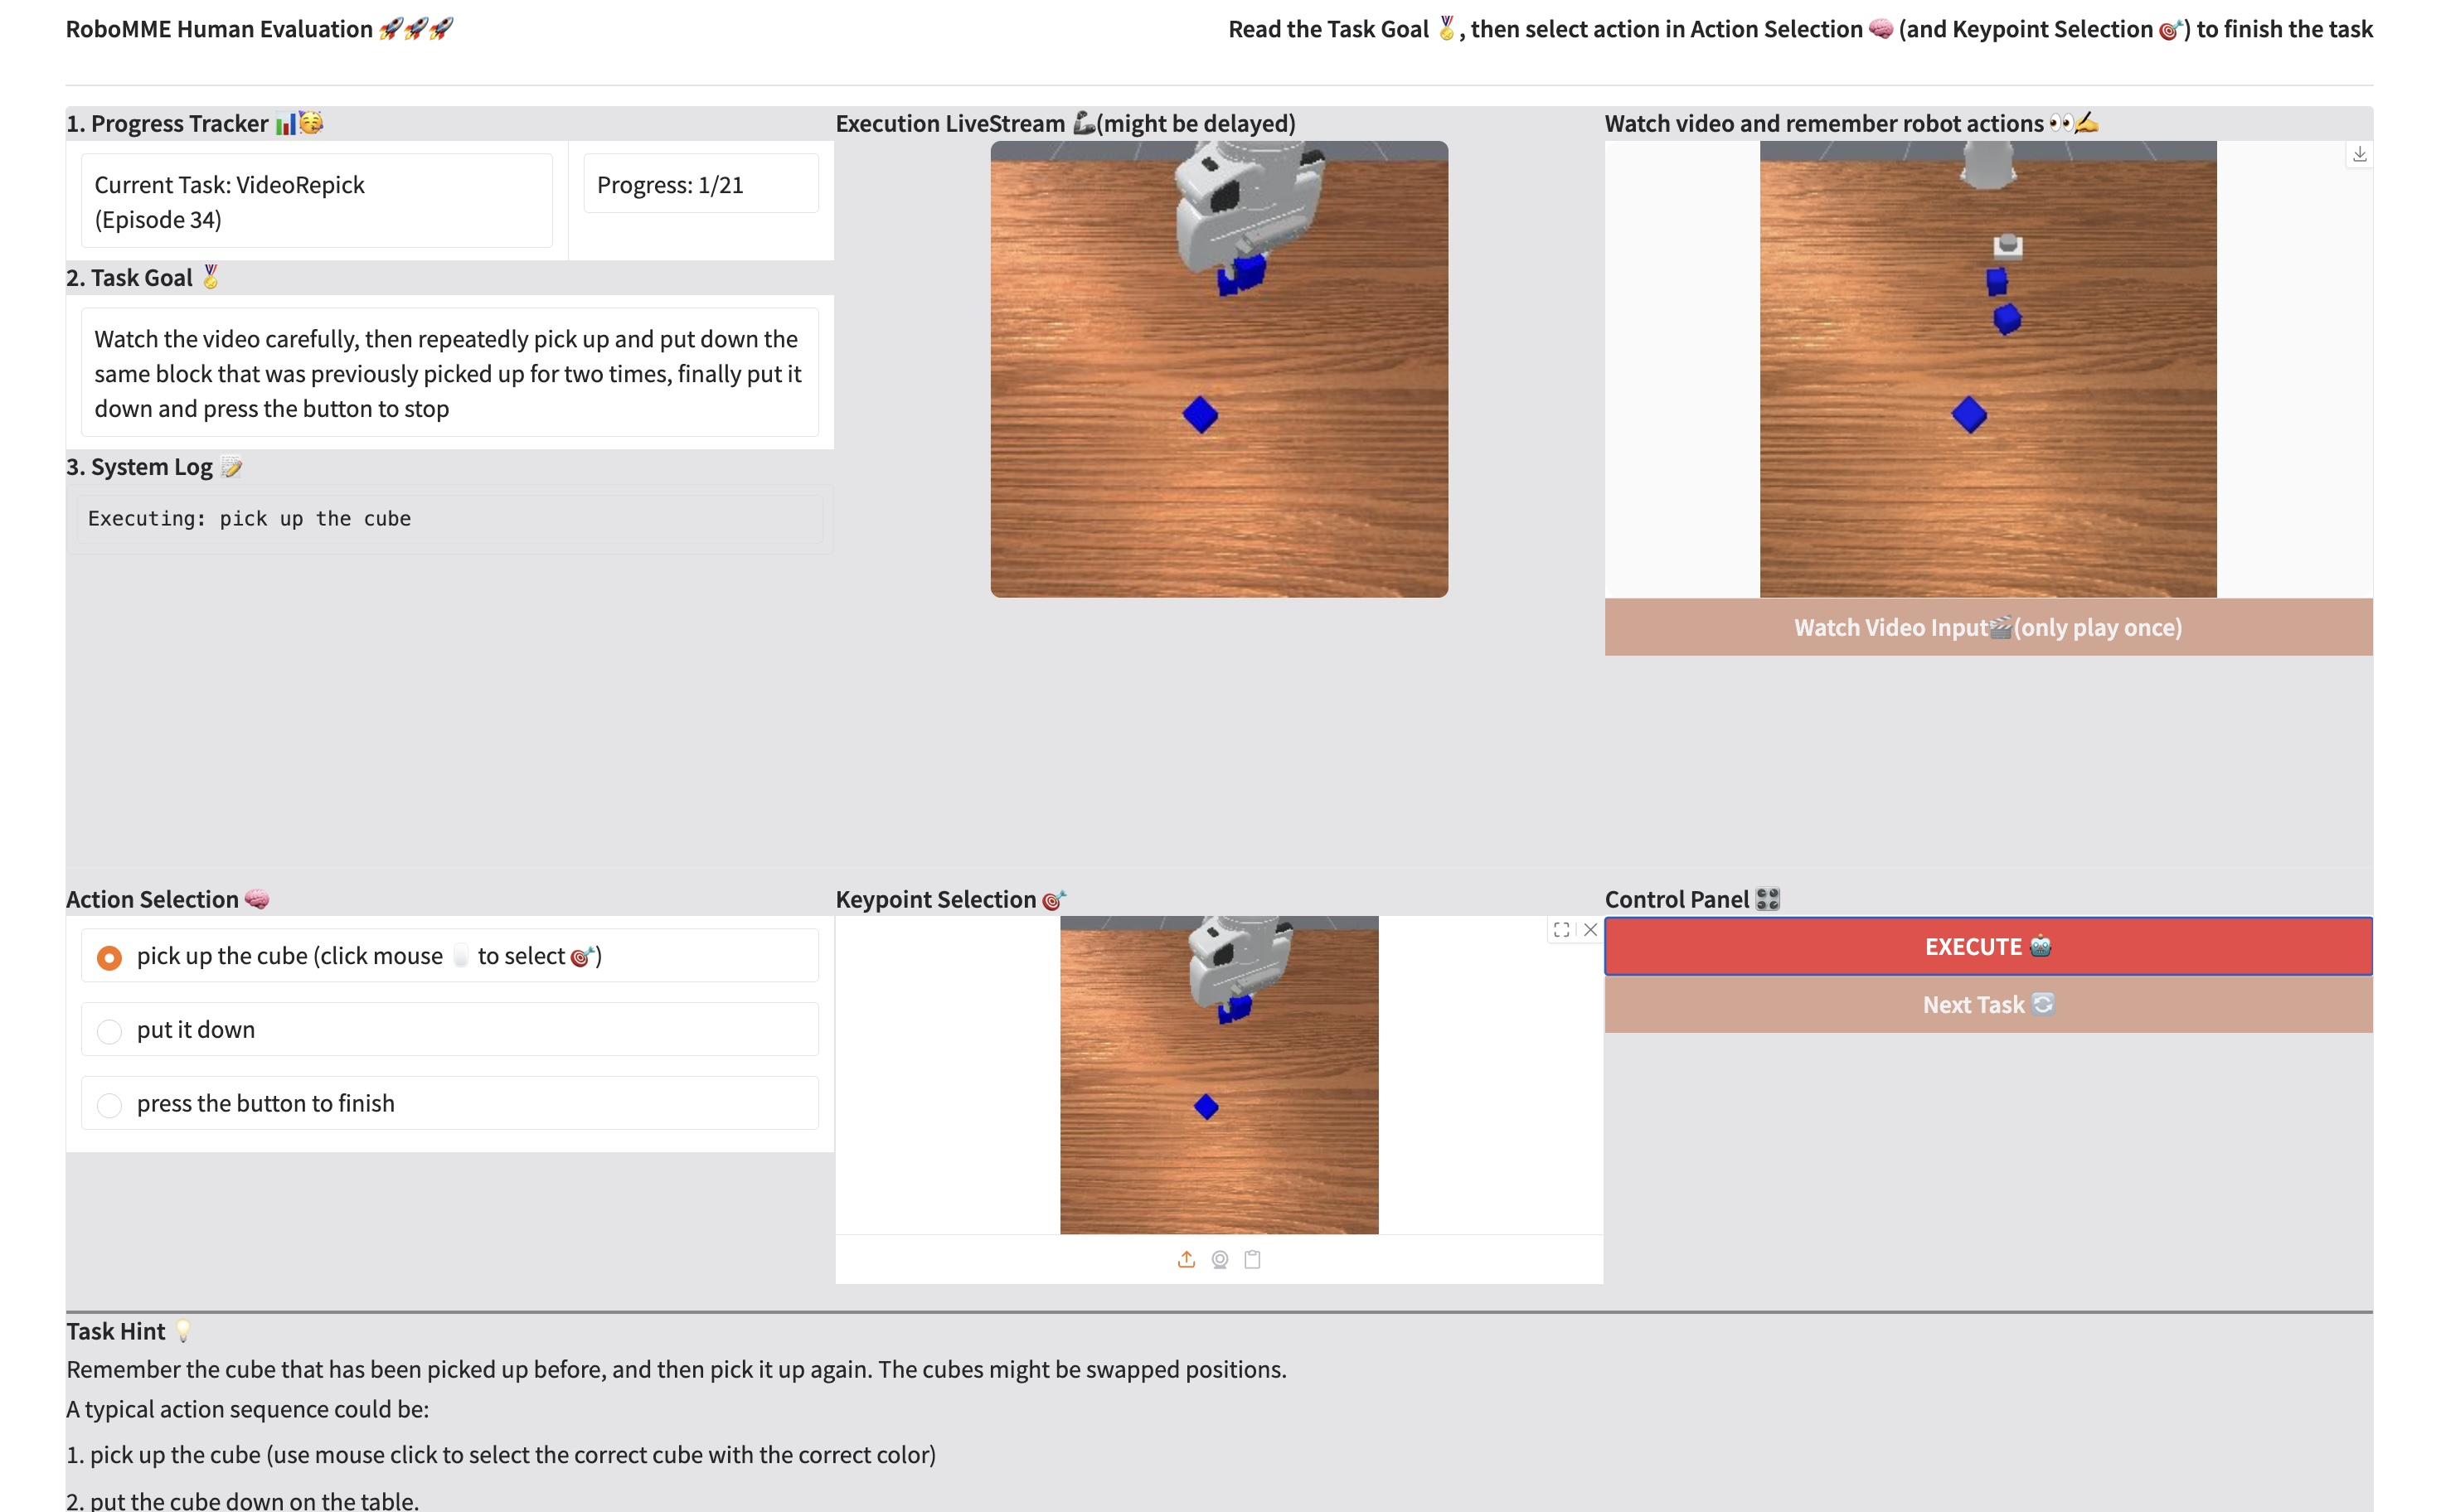
\includegraphics[width=\linewidth]{images/human_study.jpg}
    \caption{Human Study GUI.}
    \label{fig:gui}
\end{figure}


\clearpage
